%%%%%%%%%%%%%%%%%%%%%%%%%%%%%%%%%%%%%%%%%
% Masters/Doctoral Thesis 
% LaTeX Template
% Version 2.5 (27/8/17)
%
% This template was downloaded from:
% http://www.LaTeXTemplates.com
%
% Version 2.x major modifications by:
% Vel (vel@latextemplates.com)
%
% This template is based on a template by:
% Steve Gunn (http://users.ecs.soton.ac.uk/srg/softwaretools/document/templates/)
% Sunil Patel (http://www.sunilpatel.co.uk/thesis-template/)
%
% Template license:
% CC BY-NC-SA 3.0 (http://creativecommons.org/licenses/by-nc-sa/3.0/)
%
%%%%%%%%%%%%%%%%%%%%%%%%%%%%%%%%%%%%%%%%%

%----------------------------------------------------------------------------------------
%	PACKAGES AND OTHER DOCUMENT CONFIGURATIONS
%----------------------------------------------------------------------------------------

\documentclass[
11pt, % The default document font size, options: 10pt, 11pt, 12pt
oneside, % Two side (alternating margins) for binding by default, uncomment to switch to one side
english, % ngerman for German
singlespacing, % Single line spacing, alternatives: onehalfspacing or doublespacing
%draft, % Uncomment to enable draft mode (no pictures, no links, overfull hboxes indicated)
%nolistspacing, % If the document is onehalfspacing or doublespacing, uncomment this to set spacing in lists to single
%liststotoc, % Uncomment to add the list of figures/tables/etc to the table of contents
%toctotoc, % Uncomment to add the main table of contents to the table of contents
%parskip, % Uncomment to add space between paragraphs
%nohyperref, % Uncomment to not load the hyperref package
headsepline, % Uncomment to get a line under the header
%chapterinoneline, % Uncomment to place the chapter title next to the number on one line
%consistentlayout, % Uncomment to change the layout of the declaration, abstract and acknowledgements pages to match the default layout
table,
]{MastersDoctoralThesis} % The class file specifying the document structure

\usepackage[utf8]{inputenc} % Required for inputting international characters
\usepackage[T1]{fontenc} % Output font encoding for international characters

\usepackage{mathpazo} % Use the Palatino font by default
\usepackage{float}

\usepackage[backend=bibtex,style=authoryear,natbib=true,doi=false]{biblatex} % Use the bibtex backend with the authoryear citation style (which resembles APA)

\addbibresource{references.bib} % The filename of the bibliography

\usepackage[autostyle=true]{csquotes} % Required to generate language-dependent quotes in the bibliography

%----------------------------------------------------------------------------------------
%	MARGIN SETTINGS
%----------------------------------------------------------------------------------------

\geometry{
	paper=a4paper, % Change to letterpaper for US letter
	inner=2.5cm, % Inner margin
	outer=3.8cm, % Outer margin
	bindingoffset=.5cm, % Binding offset
	top=1.5cm, % Top margin
	bottom=1.5cm, % Bottom margin
	%showframe, % Uncomment to show how the type block is set on the page
}

%----------------------------------------------------------------------------------------
%	THESIS INFORMATION
%----------------------------------------------------------------------------------------

\thesistitle{Analysis of the SVM-RFE algorithm for feature selection} % Your thesis title, this is used in the title and abstract, print it elsewhere with \ttitle
\supervisor{Luis A. \textsc{Belanche}} % Your supervisor's name, this is used in the title page, print it elsewhere with \supname
\examiner{} % Your examiner's name, this is not currently used anywhere in the template, print it elsewhere with \examname
\degree{Bachelor Degree in Informatics Engineering} % Your degree name, this is used in the title page and abstract, print it elsewhere with \degreename
\author{Robert \textsc{Planas}} % Your name, this is used in the title page and abstract, print it elsewhere with \authorname
\addresses{} % Your address, this is not currently used anywhere in the template, print it elsewhere with \addressname

\subject{Computing} % Your subject area, this is not currently used anywhere in the template, print it elsewhere with \subjectname
\keywords{} % Keywords for your thesis, this is not currently used anywhere in the template, print it elsewhere with \keywordnames
\university{\href{http://www.upc.edu}{Universitat Politècnica de Catalunya}} % Your university's name and URL, this is used in the title page and abstract, print it elsewhere with \univname
\department{ \_ } % Your department's name and URL, this is used in the title page and abstract, print it elsewhere with \deptname
\group{ \_ } % Your research group's name and URL, this is used in the title page, print it elsewhere with \groupname
\faculty{Facultat d'informàtica de Barcelona} % Your faculty's name and URL, this is used in the title page and abstract, print it elsewhere with \facname

\AtBeginDocument{
\hypersetup{pdftitle=\ttitle} % Set the PDF's title to your title
\hypersetup{pdfauthor=\authorname} % Set the PDF's author to your name
\hypersetup{pdfkeywords=\keywordnames} % Set the PDF's keywords to your keywords
}

\begin{document}

\frontmatter % Use roman page numbering style (i, ii, iii, iv...) for the pre-content pages

\pagestyle{plain} % Default to the plain heading style until the thesis style is called for the body content

%----------------------------------------------------------------------------------------
%	TITLE PAGE
%----------------------------------------------------------------------------------------

\begin{titlepage}
\begin{center}

\vspace*{.06\textheight}
{\scshape\LARGE \univname\par}\vspace{0.5cm} % University name
\textsc{\Large \facname}\\[1.5cm] % Facultry name
\Large{GEP \ — \  Deliverable 2}\\[0.2cm] % Thesis type
\small{\emph{GEP tutor:} Andujar Larios}\\[0.5cm]

\HRule \\[0.4cm] % Horizontal line
{\huge \bfseries \ttitle\par}\vspace{0.4cm} % Thesis title
\HRule \\[1.5cm] % Horizontal line
 
\begin{minipage}[t]{0.4\textwidth}
\begin{flushleft} \large
\emph{Author:}\\
\href{http://www.hubbit86.com}{\authorname} % Author name - remove the \href bracket to remove the link
\end{flushleft}
\end{minipage}
\begin{minipage}[t]{0.4\textwidth}
\begin{flushright} \large
\emph{Director:} \\
\href{https://www.cs.upc.edu/~belanche/}{\supname} % Supervisor name - remove the \href bracket to remove the link  
\end{flushright}
\end{minipage}\\[4cm]

\vfill

\large \degreename\\ % Speciality name
\large Specialization:  Computing\\[0.5cm] % Speciality name

\vfill

% \large \textit{A thesis submitted in fulfillment of the requirements\\ for the degree of \degreename}\\[0.3cm] % University requirement text
% \textit{in the}\\[0.4cm]
% \groupname\\\deptname\\[2cm] % Research group name and department name

\includegraphics{logo.pdf} % University/department logo - uncomment to place it

\vfill

{\large \today}\\[4cm] % Date

\vfill
\end{center}
\end{titlepage}



%----------------------------------------------------------------------------------------
%	THESIS CONTENT - CHAPTERS
%----------------------------------------------------------------------------------------

\mainmatter % Begin numeric (1,2,3...) page numbering

\pagestyle{thesis} % Return the page headers back to the "thesis" style
\tableofcontents
\chapter{Non-linear Kernels} % Main chapter title

\label{Chapter1} % For referencing the chapter elsewhere, use \ref{Chapter1} 
\label{eq:ch4.grankingcoeff}

%----------------------------------------------------------------------------------------

This modification intends to apply the required modifications in the calculation of the ranking criteria so that non-linear kernels can be used in the SVM.

\section{Description and reasoning}
\label{sec:stopCond.desc}

When a problem is not linearly separable, we know that a hard-margin SVM will not be able to correctly place a decision boundary. In this case a soft-margin SVM may be used, but it only works to some extent and if the underlying distribution is near linearly separable. If it is not the case, much better results can be achieved by using non-linear kernels.

To use this method within SVM-RFE we must first be able to compute the ranking coefficient from a non-linear kernel. In contrast with the linear kernel case, where the ranking coefficient can be simplified to $(w_i)^2$, for non-linear kernels, however, since it is a more general case, no simplification can be performed. Instead, we use the general ranking coefficient for SVM (Equation \ref{eq:ch4.grankingcoeff}), which we restate here:
\begin{align*}
    DJ(i) = (1/2)(\boldsymbol{\alpha}^\T \vb{H} \boldsymbol{\alpha} - \boldsymbol{\alpha}^\T \vb{H}(-i) \boldsymbol{\alpha})
\end{align*}

Note that the \emph{hessian} matrix $\vb{H_{i,j}} = y_iy_jk(\vb{x_i}, \vb{x_j})$ needs be computed each iteration (since the dimension of $\vb{x_i}$ and $\vb{x_j}$ will change), and also for each feature removed in each iteration. This is slow, however various optimizations may exist, as discussed in Section [ref.].

\section{Pseudocode formalization}

\textbf{Definitions:}

\begin{itemize}
    \item $X_0 = [\vt{x_0}, \vt{x_1}, \dotsc, \vt{x_k}]^T$ list of observations.
    \item $\vt{y} = [y_1, y_2, \dotsc, y_k]^T$ list of labels.
\end{itemize}

\begin{algorithm}[H]
    \DontPrintSemicolon
      \KwInput{$t, k$ \tcp*{$t$ = step, $k$ = kernel function}}
      \KwOutput{$\vt{r}$}
      \KwData{$X_0,\vt{y}$}
      $\vt{s} = [1,2, \dotsc, n]$ \tcp*{subset of surviving features}
      $\vt{r} = []$ \tcp*{feature ranked list}
      \While{$|\vt{s}| > 0$}
        {
            \tcc*[h]{Restrict training examples to good feature indices}\\
            $X=X_0(:,\vt{s})$\VS

            \tcc*[h]{Precompute hessian matrix}\\
            $\vb{H_{i,j}} = y_iy_jk(\vb{x_i}, \vb{x_j}) \qquad \text{for all} \qquad \vb{x_i}, \vb{x_j} \in X$\VS

            \tcc*[h]{Train the classifier}\\
            $\vt{\alpha} = \texttt{SVM-train(} X, y, k \texttt{)}$\VS

            \tcc*[h]{Compute the ranking criteria}\\
            $\vt{c} = [c_1, c_2, \dots, c_{|\vt{s}|}]$ \\
            \For{$c_l \in \vt{c}$}{
                \tcc*[h]{Compute new hessian with the feature $l$ removed}\\
                $\vb{H_{i,j}}(-l) = y_iy_jk(\vb{x_i}, \vb{x_j}) \qquad \text{for all} \qquad \vb{x_i}, \vb{x_j} \in X(-l)$\VS
    
                \tcc*[h]{Calculate ranking coefficient}\\
                $c_l = (1/2)(\boldsymbol{\alpha}^\T \vb{H} \boldsymbol{\alpha} - \boldsymbol{\alpha}^\T \vb{H}(-l) \boldsymbol{\alpha})$
            }\VS

            \tcc*[h]{Find the $t$ features with the smallest ranking criterion}\\
            $\vt{f} = \texttt{argsort}(\vt{c})(\ :t)$\VS

            \tcc*[h]{Iterate over the feature subset}\\
            \For{$f_i \in \vt{f}$}{
                \tcc*[h]{Update the feature ranking list}\\
                $\vt{r} = [\vt{s}(f_i), ...\vt{r}]$\VS
    
                \tcc*[h]{Eliminate the feature selected}\\
                $\vt{s} = [...\vt{s}(1:f_i - 1), ...\vt{s}(f_i + 1:|\vt{s}|)]$
            }
        }
    \caption{SVM-RFE with Stop Condition}
    \label{alg:svmrfe-stopcond}
\end{algorithm}

\section{Results}


% Chapter 1

\chapter{Project Planning} % Main chapter title
\label{Chapter2} % For referencing the chapter elsewhere, use \ref{Chapter1} 

\newcommand{\tabhead}[1]{\textbf{#1}}

%----------------------------------------------------------------------------------------

This thesis is worth 15 ECTS credits, each of which with an estimate cost of 25 to 30 hours. Therefore, the total time allocated for this project, as indicated by the faculty, is of 375 to 450 hours. This time is to be distributed in 100 days, from 03/08/21 to 06/15/21, with an estimated work of 4 to 5 hours a day. The date of the oral defense is planned for the first week of July, this sets the deadline to be on the 06/18/21.

An extra 3 ECTS credits are to be used for project managment, this is roughly 80 hours, which makes the total time estimate for the whole project (Theisis + Project Managment) to be at best 450 hours and at worse 540 hours. In order to make a proper plannification, we have defined the estimated cost to be at 500 hours.

\section{Task definition}

In this section it is presented all the tasks that will be carried out along the project. For each, a description, duration and a list of dependencies with other tasks are given.

Project management is a mandatory group of such tasks, albeit not very useful, considering that: One, this project is done by a single individual, with assistance from a project director; And two, this is a research project, which makes planning of specific tasks difficult, since it is the results from the research that drive the next steps to be done.  

\begin{itemize}
    \item \textbf{Context and scope:} We have to indicate the general objective(s) of the project, contextualize it and justify the reason for selecting this subject area.
    \item \textbf{Project planning:} This will help us not lose focus while we're working on the project.
    \item \textbf{Budget and sustainability:} For this specific project, this is irrelevant. The budget required is negligible and already defrayed; and the impact, beyond trivial matters, is likely zero and otherwise unknown. 
    \item \textbf{Final project definition:} Review the work done in the project management tasks.
    \item \textbf{Meetings:} Online meetings are scheduled once every two weeks with the tutor of the project. Discussion of the status and next tasks to do will be done.
\end{itemize}

This project is research focused. Therefore, before starting the practical tasks research on the various topics needs to be done. This will involve collecting and analyzing previous studies that tried new methods and extensions to the SVM-RFE algorithm. We will also have to document ourselves in the SVM and feature selection areas, as well as the algorithms and the statistical theory used in the studies. Some basic understanding of bioinformatics may also be required considering the use case of most if these studies.

\begin{itemize}
    \item \textbf{Research} previous work on the literature on extensions of the algorithm and create a short \textbf{report} with the findings.
    \item Write the algorithm formalization in pseudocode.
    \item Define the expected advantages or disadvantages of this method over the base SVM-RFE.
    \item Compute the space and time complexities.
\end{itemize}

Once the initial research is done the algorithm must be codified and tested. This group is composed of the following tasks:

\begin{itemize}
    \item \textbf{Program the base SVM-RFE algorithm.} For this we will use a library for the SVM. For the RFE part, since we need to be able to extend the algorithm, we will program it from scratch.
    \item \textbf{Program the extensions of the SVM-RFE algorithm} based on the research done and the pseudocode.
    \item \textbf{Test the new extensions with artificial data.} This requires creating models and testing their performance with artificial data sets.
    \item \textbf{Obtain data sets with real data.} Multiple papers refer to publically available data-sets, we could use those and compare our results.
    \item \textbf{Test the new extensions with real data.} This requires creating models and testing their performance with real data sets.
    \item \textbf{Analyze the results} obtained in the experiments and draw conclusions. A report will be made for reference during the final documentation.
\end{itemize}


Once finished, the final documenting phase will begin. Firstly, we will collect all the information obtained in the experimental and analysis part, which will be available in the form of the reports that we've done along the tasks. Afterwards, we can start writing the documentation of the project. This will include a fairly extensive review on concepts related to SVM, statistics, feature selection and RFE. Finally, we will have to prepare for the oral defense of the project.

\begin{table}
\centering
\begin{tabular}{l l l l}
\toprule
\tabhead{ID} & \tabhead{Description} & \tabhead{Hours} & \tabhead{Dependencies} \\
\midrule
\rowcolor{gray!10} T1 & Project Managment & 80 &  \\
T1.1 & Context and Scope & 20 & T2.1  \\
T1.2 & Project planning & 10 & \\
T1.3 & Budget  and  sustainability & 10 & T1.2 \\
T1.4 & Final project definition & 20 & T1.1, T1.2, T1.3  \\
T1.5 & Meetings & 20 &  \\
\rowcolor{gray!10} T2 & Theoretical Part & 160 &  \\
T2.1 & Research & 90 &  \\
T2.2 & Formalize & 20 & T2.1  \\
T2.3 & Analyze & 50 & T2.2 \\
\rowcolor{gray!10} T3 & Practical Part & 160 &  \\
T3.1 & Program the base SVM-RFE algorithm & 10 & T2.1  \\
T3.2 & Program the extensions & 50 & T2.1, T3.1  \\
T3.3 & Test with artificial data & 20 & T3.2  \\
T3.4 & Test with real data & 30 & T3.2  \\
T3.5 & Analyze  the  results & 50 & T3.3, T3.4 \\
\rowcolor{gray!10} T4 & Documentation & 100 &  \\
T4.1 & Writte the documentation & 80 & T2, T3  \\
T4.2 & Prepare the thesis defense & 20 & T4.1  \\
\bottomrule\\
\end{tabular}
\caption{Summary and time estimates of the tasks.}
\label{tab:tasks}
\end{table}

\begin{figure}[H]
    \centering
    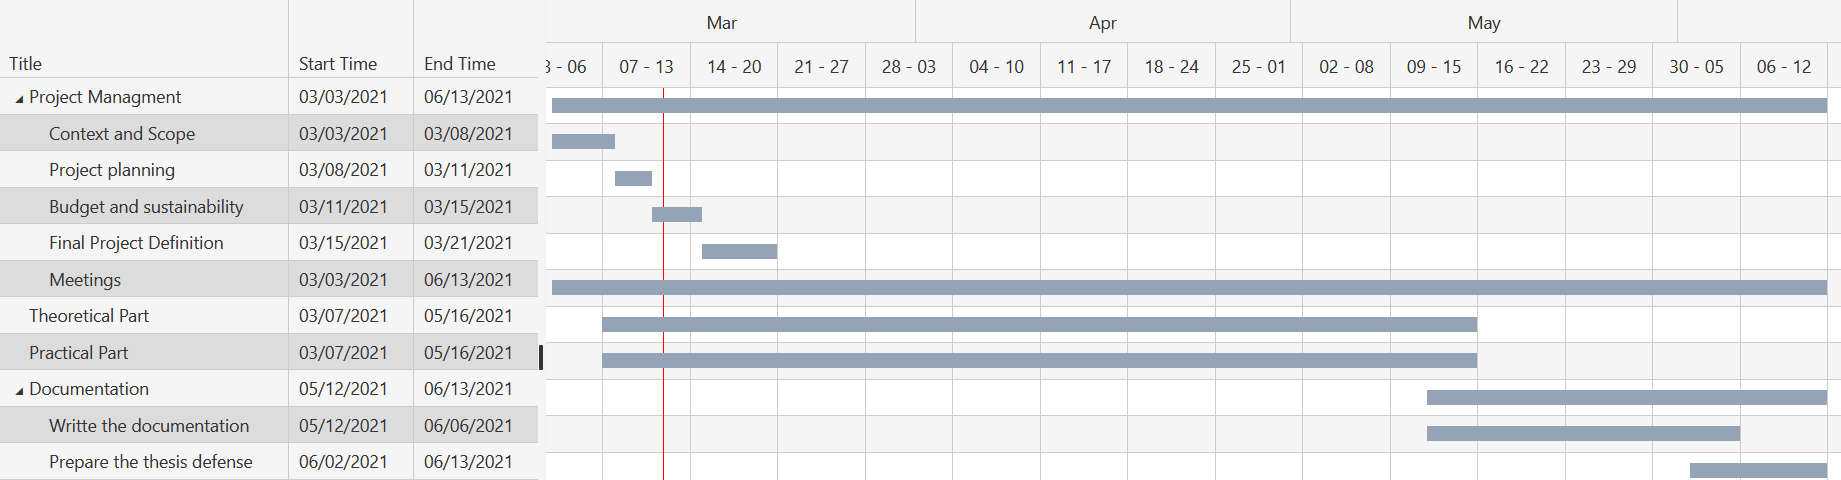
\includegraphics[scale=0.35]{gantt.png}
    \caption{A summary of the tasks represented with a gantt chart. Notice that all the theoretical and practical tasks are done in parallel.}
    \label{fig:gantt}
\end{figure}

\section{Resources}

Our project needs resources to carry out its correct development. These resources have been divided in 4 different groups: human, hardware, software and material resources.

\subsection{Human resources}

There are three human resources that are directly involved in this project.

\begin{itemize}
    \item \textbf{The researcher:} He is responsible for the development of the project, that is, he will have to plan, analyze, program, experiment and document the project.
    \item \textbf{The director/tutor:} He is responsible for leading and guiding the researcher for the correct development of the project.
    \item \textbf{The GEP tutor:} He is in charge of reviewing the project management tasks done in the initial stage of the project.
\end{itemize}

\subsection{Hardware Resources}

The most essential resource needed is a computer connected to the internet. In this project a personal computer will be used. Its specializations are 16 GB of RAM and a CPU \emph{AMD Ryzen 7 4800HS}, with a base speed of 2.9 GHz and 8 cores. Hardware required for a connection to the internet (a router, an access point, etc) is also taken into account.

\subsection{Software Resources}

For project management tasks \texttt{Google Calendar} will be used. A number of other Google products such as \texttt{Google Mail}, \texttt{Google Drive} or \texttt{Google Meet} will also be used as tools required for communication with the director or storing of information.

The documentation will be written in \LaTeX, a document preparation system often used in academia. It has the advantage to integrate well with version control systems. A \LaTeX \ template named "\texttt{Masters/Doctoral Thesis}" will be used to facil\-itate the type\-setting and styling of the document. This template was made by Vel and Johannes Böttcher and licensed under \texttt{LPPL 1.3}, based on previous work from Steve R. Gun and Sunil Patel and used with minor modifications. The original is available at \url{http://www.latextemplates.com/}. The document will be written with the \texttt{Microsft Visual Studio Code} editor, using the \texttt{LaTeX Workshop} extension, and it will be compiled with the \texttt{MiKTex} distribuition installed on a \texttt{Linux} machine run\-ning virtualized within a \texttt{WSL} container on top of the actual operating system, a \texttt{Microsoft Windows 10}. For browsing the internet the latest available version of the \texttt{Firefox} web browser will be used, and references to papers will be kept with the \texttt{Zotero} reference manager.

For the practical part, the programming language of choice will be \texttt{Python3}. This is currently one of the programming languages with better popularity in machine learning and related applications. Various libraries and software packages will be used for different tasks. For parsing datasets the \texttt{pandas} library will be used. For data visualization the \texttt{mathplotlib} library will be used. Also, a general tool-set designed for machine learning, the library \texttt{sklearn}, will be used. Finally, code will be documented in-place during its development with the \texttt{Jupyter Notebook} software.

Other libraries and software packages could also be used if the need arises. 

\section{Risk Management}

The potential risks and obstacles have already been introduced in section \ref{sec:risk}. In this section we will focus on a contingency plan to mitigate the risks.

\begin{itemize}
    \item \textbf{Deadline of the project:} The flexibility of the Kanban methodology should help us modify our schedule and working hours if required. If it becomes apparent that the deadline will not be meet, an extension of the deadline can be requested.
    \item \textbf{Bugs on some libraries:} Alternative libraries can be used. If no alternative is found, because most of the used libraries are open source, a \emph{bugfix} could be implemented.
    \item \textbf{Insufficient computational power:} This can be mitigated by using a small sample of the data-set. This though, can induce a small performance reduction, and thus make the results not comparable with each other. 
    \item \textbf{Hardward related issues:} To avoid it data loss, all code and documentation will be routinely uploaded to the cloud in a \texttt{GitHub} repository and \texttt{Google Drive} account.
\end{itemize}





%----------------------------------------------------------------------------------------
%	BIBLIOGRAPHY
%----------------------------------------------------------------------------------------

\printbibliography[heading=bibintoc]

%----------------------------------------------------------------------------------------

\end{document}  
